\documentclass[ngerman]{scrartcl}

\usepackage[utf8]{inputenc}
\usepackage{babel}
\usepackage[T1]{fontenc}
\usepackage{lmodern}
\usepackage{color}
\usepackage{graphicx}
\usepackage[colorlinks=true, linkcolor=cyan]{hyperref}
\usepackage{enumerate}
\usepackage{amsmath}
\usepackage{braket}
\usepackage{placeins}
\usepackage{amsfonts}

\newcommand{\erw}[1]{\langle {#1} \rangle}
\newcommand{\Hil}{\mathcal{H}}
\newcommand{\diff}{\mathrm{d}}

\usepackage[backend=bibtex, style=numeric-comp, sorting=nty]{biblatex}
\bibliography{mybib}

\begin{document}
 
	\begin{titlepage}
		\begin{minipage}[c][\textheight][c]{\textwidth}
			\begin{center}
				{ \Huge \textbf{Thermodynamik schwarzer Löcher} }
				
				\vspace*{1cm}
				{\large eine Seminararbeit von}
				
				\vspace*{0.2cm}
				{\Large Tamara Szecsey}
				
				\vspace*{1cm}
				{\large \today}
				
				\vspace*{4cm}
				\hspace*{1cm} 
\includegraphics[height=30ex]{LOGO_UR}
			\end{center}
		\end{minipage}
	\end{titlepage}
	
\tableofcontents
\newpage
\section{Einleitung}
Was ist Thermodynamik?

\section{Informationsentropie im Allgemeinen} \label{InfoentropieAllg}
Zunächst ein kurzer Einblick, um welche Art von Entropie es sich hier handeln wird. Ludwig Boltzmann hatte festgestellt, dass eine Proportionalität zwischen der Entropie $S$ und $\log W$ herrscht, wobei $W$ die Wahrscheinlichkeit darstellt. Der zugehörige Proportionalitätsfaktor $k$ ist die Boltzmann-Konstante.
	\begin{align}
		S &= k \log W
	\end{align}
Dies ist eine wichtige Verbindung zwischen Statistik und Thermodynamik. 
Die Verallgemeinerte Boltzmannsche Beziehung bring dann die sogenannte Informationsentropie hervor, die in diesen Gestalten geschrieben werden kann:	
	\begin{align} \label{Informationsentropie}
		S &=
		\left\{
		\begin{aligned}
		&- k ~\erw{\,\ln \rho\,} \\
		&-k~ Sp(\rho \ln \rho) \\
		&-k \sum_n \rho_n \ln \rho_n
		\end{aligned}
		\right.
	\end{align}
wobei $\rho$ die Wahrscheinlichkeit ist, die Energie $E_n$ im mikrokanonischen Ensemble anzutreffen. 
(Wir wollen hier nicht weiter auf die thermodynamische Definition der Entropie eingehen, für Fragen zu den Grundlagen siehe \cite{Brenig})

Wie wir jetzt aber zu Information kommen, soll ein Beispiel zeigen. Dabei geht es um eine quantitativen Betrachtung der selben.
Wir betrachten nun eine Reihe von Ereignissen $E_n (n = 1, 2, \ldots, N)$, die mit bestimmten Wahrscheinlichkeiten $\rho_n$ auftreten, wobei
	\begin{align*}
		\sum_{n=1}^N \rho_n &= 1
	\end{align*}
Nun sehen wir das Eintreten bestimmter die Ereignisse $E_n$, dabei hat jede unserer Feststellungen hat einen Informationswert $I_n$. Nach häufiger Wiederholung kann man einen mittleren Informationsgehalt aufstellen:
	\begin{align*}
		I = \sum_{n=1}^N \rho_n I_n
	\end{align*}
Hier legen wir wie in der Informationstheorie fest
	\begin{align*} \label{Informationsgehalt}
		I = - \sum \rho_n \mathrm{ld}(\rho_n)
	\end{align*}
wobei $\mathrm{ld}(x)$ der dyadische Logarithmus von $x$ ist, also $2^{\mathrm{ld}(x)} = x$. 
Wir haben \eqref{Informationsgehalt} so festgelegt, dass ein Ereignis allein durch eine Ja oder Nein Frage (oder durch 0 und 1) vollständig charakterisierbar ist. 
Dass unserer mittlerer Informationsgehalt unserer Entropie von \eqref{Informationsentropie} ähnlich sieht, ist kein Zufall.

Wir machen nun zwei Zahlenbeispiele zur Veranschaulichung:
	\begin{itemize}
		\item[\textit{1.\,Beispiel:}] Sei $N=2, \rho_1 = \rho_2= \frac{1}{2}$ was sein könnte: Ein Teilchen hält sich mit gleicher Wahrscheinlichkeit in der linken oder rechten Hälfe eines Kastens auf, oder Zahl und Wappen für ein Münzwurf.
		Es benötigt Ja-Nein-Frage, um herauszufinden, wo das Teilchen liegt oder wie herum die Münze gefallen ist.
			\begin{align*}
				I = \mathrm{ld}(2) = 1 \,\mathrm{bit}
			\end{align*}
		Ein bit ist die Einheit für Information.
		\item[\textit{2.\,Beispiel:}]Sei $N=6, \rho_n = \frac{1}{6}$, wobei die Ereignisse $E_n$ die Seiten eines Würfels sein könnten, der Informationsgehalt
			\begin{align*}
				I = \mathrm{ld}(6) &= 2,58 \,\mathrm{bit}
			\end{align*}
	\end{itemize}
(siehe auch \cite{Brenig})

\section{In Bezug auf die thermodynamischen Hauptsätze}
	\subsection{Nullter Hauptsatz der Thermodynamik}
%Temperatur müssen wir definieren können
	Wir beginnen mit der Erklärung der Hawkingstrahlung. Diese fand Steven Hawking \cite{ParticleCreation}, als er den gekrümmten Raum in euklidische Koordinaten transformierte (z.B. Minkowski-Raum). Hierbei entstanden im Grundzustand Entartungen, die störungstheoretisch entwickelt werden müssen. 
	
	Anschaulich bedeutet dies, dass zwei verschränkte Teilchen (siehe Appendix \ref{Verschränkung}), die durch Vakuumfluktuation am Horizont des schwarzen Lochs entstehen so getrennt werden, dass das mit negativer Energie in das schwarze Loch hinein fällt, und das, welches eine positive Energie besitzt ins Unendliche im Raum verschwindet. 

%Temperaturgleichgewicht: so viel abstahlen wie aufnehmen -> nullter HS der Thermodynamik
%SH beschleunigung auf der Oberfläche

	\subsection{Erster Hauptsatz der Thermodynamik}
%Innere Energie dU

	\subsection{Zweiter Hauptsatz der Thermodynamik}
%zweiter HS Fläche proto Entropie, hier holographisches Prinzip
%ganzes Universum, sehr verallgemeinert worden (Bousseau)
%bilder zwei schwarze löcher vereinigen M_3 > M_2 + M_1 usw.
	\subsubsection{Das holographische Prinzip}
	Wir befinden uns in der String Theorie in einem flachen Raum. Wir schauen nun auf eine Region $\Gamma$ in so Einem. 
	
	Die maximale Entropie aller physikalischen Systeme, die in $\Gamma$ hinein passen, sind proportional zur Fläche des Rands $\partial \Gamma$, welche in Planck Einheiten aufgeteilt ist. 
	
	Typischerweise, bei einem Gitter aus Spins, misst die Maximalentropie die einfachen Freiheitsgrade, also wie oben erwähnt so etwas wie den Spin oder Fermionen. Außer in der Gravitationssystemen ist dies proportional zum Volumen $\Gamma$. 
	
	Diese obere Grenze der Entropie sagt uns, dass die maximale Anzahl der sich unterscheidenden Freiheitsgrade proportional zur Fläche ist. Das bedeutet allerdings für große makroskopische Regionen eine enorme Verminderung die Freiheitsgrade. Bei einer Dimension $L$ skaliert die Anzahl der Freiheitsgrade pro Volumen mit $\frac{1}{L}$ in Planck Einheiten.
	Wenn wir $L$ groß genug machen, werden die Freiheitsgrade also sehr dünn besiedelt im Raum verteilt sein. Allerdings wollen wir immer noch alle mikroskopischen Prozesse erfassen, die irgendwo in der Region passieren. 
	
	Eine Art und Weise dies zu betrachten ist mit Freiheitsgraden von $\Gamma$, welche alle auf $\partial \Gamma$ leben, mit einer Dichte nicht größer als $\sim 1$ Freiheitsgrad pro Planckfläche. In anderen Worten, wir beschreiben einen dreidimensionalen Raum, nämlich die Kugel um das schwarze Loch mit dem Horizontradius durch ein zweidimensionales Hologramm an der Grenze! Dies nennt man Holographisches Prinzip. 
	
	\begin{figure} 
		\begin{center}
			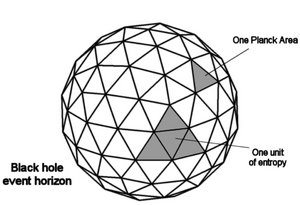
\includegraphics[width=0.6\textwidth]{BHentropy1}
		\end{center}
		\caption{Zweidimensionale Oberfläche des Horizonts aufgeteilt in Planck Einheiten. Die Entropie hat allerdings eine Einheit von 4 solchen Planckflächen für ein Bit. Siehe \ref{BHEntropie}. (aus \cite{BekensteinHawking})}
	\end{figure} 

\FloatBarrier
\section{Evaporation \checkmark}
Stephen Hawking hat in seinem Paper \cite{ParticleCreation} gezeigt, dass ein großes schwarzes Loch für einen Beobachter in großer Ferne eine Temperatur besitzt:
	\begin{align}
		T_{\text{Hawking}} = \frac{\hbar c^3}{8 \pi GM}
	\end{align}
Nun bedeutet dies eine gewisse Wärmestrahlung, welche von jedem schwarzen Loch ausgeht also ein Energieverlust. Dank Einstein wissen wir, dass Masse und Energie sich gleichen, wenn man c = 1 setzt. Jedes schwarze Loch verliert also im Lauf der Zeit an Masse, bis es verdampft. Dieser Vorgang wird als Evaporation bezeichnet. Nach einigen Rechnungen, siehe z.B. \cite{JerusalemsLectures}, erfahren wir, dass
	\begin{align}
		t_{\text{evap}} \sim G^2 M^3
	\end{align}
Ein sonnenschweres schwarzes Loch würde nach etwa $10^{66}$ Jahren verdampft sein (zum Vergleich, das alter unseres Universums wird auf $13,8 \cdot 10^{9}$ Jahre geschätzt). Man hätte ein riesen Problem dies nachzuweisen, vielleicht wenn wir herausfinden, wie wir kleinere schwarze Löcher produzieren können. 

Aber was passiert mit der Entropie?
Hawking \cite{BreakdownGravitationalCollapse} legte dar, dass die Vorstellung, die Entropie würde die Anzahl der Möglichkeiten zählen, wie ein schwarzes Loch entstehen könne, gegen die Quantenmechanik verstößt.
Außerdem wird das schwarze Loch beim verdampfen bevor es komplett verschwindet erst Plancksche Größen annehmen, in der unsere bekannten physikalischen Gesetze vermutlich nicht mehr gelten. 

Eine von den zwei folgenden Ereignissen muss passieren:
	\begin{enumerate}[(1)]
		\item Die Verdampfung stoppt und das schwarze Loch in Planckgröße bleibt weiter unverändert im Raum. Dieses Überbleibsel hat eine sehr hohe Verschränkungsentropie weil es mindestens die gesamte Entropie des schwarzen Lochs vor dem Beginn der Verdampfung beinhalten muss. \label{1}
		
		\item Die Verdampfung wird zu Ende geführt. Die Energieerhaltung verhindert, dass mit dem letzten Ausstoß von Photonen genug Verschränkungsentropie mitgetragen werden kann, damit diese Zustände zusammen mit denen der zuvor ausgestrahlten Strahlung wieder einen reinen Zustand bilden können. Dies verletzt die Quantenmechanik, das Endresultat ist ein Mischzustand mit Entropie in der Größenordnung des Horizonts in Planckgrößen ganz am Anfang.  \label{2}
	\end{enumerate}
Punkt (\ref{1}) ist zwar Möglich, aber wenn ein schwarzes Loch aus Photonen und Gravitonen entsteht, dann muss es sich auch komplett wieder in diese auflösen können (es wäre also Inkonsistent mit der CPT(charge, parity, time = Ladung, Parität, Zeit)).

Unter Anderem Hawking plädieren für Punkt (\ref{2}). Er meint, dass die Entstehung und Verdampfung eines schwarzen Lochs nicht mit einer unitären S-Matrix beschrieben werden kann, also dass schwarze Löcher quantenmechanische und klassiche Information zerstören kann. 

Wem das nicht gefällt, der würde eher für einen dritten Punkt stimmen:
	\begin{enumerate}[(3)]
		\item Die Hawkingstrahlung kommt genau genommen nicht in einem Mischzustand. Die Information wird in den Verbindungen zwischen Hawkingphotonen hinausgetragen. Am Ende der Verdampfung haben wir wieder einen reinen Zustand des Strahlungsfeldes. Nur kleine Untersysteme sehen so aus, als wären sie thermisch, deshalb funktioniert diese Betrachtungsweise nur, wenn wir nicht auf zu viele Photonen zugleich schauen. 
	\end{enumerate}   
(Bei weiterer Interesse, bitte siehe Jerusalem Lectures \cite{JerusalemsLectures})

	
	\section{Die Entropie des schwarzen Lochs in Formeln}
	Masse, elektrische Ladung und Drehmoment sind in der gleichen Kombination immer proportional zur Oberfläche des schwarzen Lochs. Sowohl Hawking also auch Misner, Thorne und Wheeler haben gezeigt, dass sein Ereignishorizont nicht kleiner werden kann, meistens wird er sogar größer.
	
	Diese Oberfläche verhält sich sozusagen wie die thermodynamische Entropie in geschlossenen Systemen. 
	Durch die Hawkingtemperatur \cite{ParticleCreation} und der Definition von Temperatur in der Thermodynamik
		\begin{align}
			\frac{\diff S}{\diff E} &= \frac{1}{T},&
			T_{\text{Hawking}} &= \frac{\hbar c^3}{8 \pi G M}
		\end{align}
	und durch ersetzen von $E = Mc^2$, erhalten wir
		\begin{align} \label{SHentropie}
			S_{BH} &= \frac{c^3 A}{4 G \hbar} = \frac{A}{4 L_P^2} 
		\end{align}
	Der Horizont ist an Fläche $A$, welche eine Kugeloberfläche um das schwarze Loch mit dem Schwarzschildradius bildet:
		\begin{align}
			r_h &= \frac{2 GM}{c^2} ,& A = 4 \pi r_h^2 
		\end{align}
	Ein sonnen-schweres schwarzes Loch hätte eine Horizontfläche $\frac{1}{5}$-mal so groß wie die Erdoberfläche und ihre Entropie wäre von der Ordnung $10^{77}$. Dies ist über zehn Größenordnungen höher, als die Entropie der jetzigen Sonne.  
	
	Es scheint also, dass die Entropie des schwarzen Lochs nicht mit der hineingefallenen Entropie während seiner Entstehung verglichen werden kann.	
	
\section{Weitere Betrachtungen}
	\subsection{Wirkungsintegrale}
	\subsection{Loop Quantum Gravity (LQG)}	%geht nicht in ART, CPT falsch
Die Loop-Quantengravitation (Loop = Schleifen) ist eine Konkurrenztheorie der Stringtheorie und nimmt keine Singularität in der Mitte des schwarzen Lochs an, sondern beinhaltet die Theorie, dass es weiße Löcher gibt, die sich wie schwarze Löcher verhalten, nur das die Zeit rückwärts läuft. 

Ein einlaufendes Wellenpaket würde dann, während es einem 'Quantum bounce' durchmacht, durch das schwarze Loch in ein weißes Loch hineintunneln. Die Metrik, die Rovelli und Haggard \cite{LQGRovelli} aufgestellt haben, werde ich hier nun kurz anschneiden.
%Hier kommen damit korrekturen 

%nur Quantenmechanik sagen, Information kann nicht verloren geht

\appendix
\section{Verschränkung} \label{Verschränkung}
	Durch die Quantenfluktuation im Vakuum, die durch die Heisenbergsche Unschärferelation auch erlaubt ist, können Teilen und Antiteilchen für kurze Zeit sozusagen aus dem Nichts entstehen und wieder verschwinden. Dabei sind genau diese Teilen verschränkt.
	\\ \\
	Was das genau bedeutet erkläre ich nun Anhand eines einfacheren Beispiels:
	
	Sagen wir, wir besitzen zwei Kugeln, welche die Farben blau oder rot haben können. Sie können allerdings nicht die gleiche Farbe haben. 
	Zu Beginn wissen wir nicht, welche Kugel welche Farbe hat, sie stecken z.B. in zwei separaten Kisten. Wir nennen die Kugeln $K_1$ und $K_2$ und entfernen Sie voneinander, sodass wir nur noch $K_1$ in einer Kiste vor uns haben. 
	
	Wenn wir nun die Kiste öffnen, wissen wir nicht nur, welche Farbe $K_1$ hat, sondern auch, dass die Kugel $K_2$, die wir im Moment nicht sehen können, genau die andere Farbe hat! 
	
	Solange wir aber die Kisten nicht öffnen, befinden sich die Kugeln in einem verschränkten Zustand, in dem zwar beide Farben möglich sind, aber die Farben voneinander abhängen. 
	
	Das bedeutet allerdings nicht, dass so Information übertragen werden kann. Entfernen wir z.B. die zweite Kugel bis zum anderen Ende der Milchstraße, so wissen wir beim Öffnen unserer Kiste welche Farbe die Kugel auf am anderen Ende hat, aber die Person, die dort steht wird das erst erfahren, wenn sie selbst die Kiste öffnet oder wir ein Signal dort hingeschickt haben.

\section{Zustände in der Thermodynamik}

\subsection*{Mikrozustand}
Ein Mikrozustand ist im klassischen Fall ein Punkt im Phasenraum. Damit ist Ort und Impuls für jedes Teilchen gegeben.

\subsection*{Makrozustand}
Viele Mikrozustände bilden einen Makrozustand, der durch Parameter dargestellt ist, die nicht mehr direkt mit Ort oder Impuls einzelner Teilchen zu tun hat. 


\newpage
\printbibliography
%\printindex
\end{document}